\chapter{Hyperbolic geometry}\label{hyperbolic}
We introduce hyperbolic spaces by putting them in contrast with the Euclidean space we are more accustomed to~\cite{Iversen1992hyperbolicGeometry}.
A simple set of axioms for a plane geometry can be presented in the framework of metric spaces. By a \term{line} in a metric space $X$ we intend the image of the real number line., expressed though a distance preserving map $\gamma: \mathbb{R}\to X$.
The three axiom of plane geometry are listed below.
\begin{description}
    \item[Incidence axiom]  Through two distinct points in $X$ there passes a unique line. The space $X$ has at least one point.
    \item[Reflection axiom] The complement of a given line in $X$ has two connected components. There exists an isometry $\sigma$ of $X$ which fixes the points of the line but interchanges the two connected components of its complement.
    \item[Parallel axiom] Through a given point $P$ outside a given line $\ell$ there passes a unique line which does not intersect $\ell$. 
\end{description}

It is possible to obtain internally consistent models of geometries which obey to all axioms except for the parallel axiom. One way to do this might be to insist that any two lines intersect. This gives rise to so called \term{Elliptic Geometry}. Another way of obtaining a non-Euclidean geometry is to state that the line through point $P$ that does not meet $\ell$ is not unique. This determines \term{Hyperbolic Geometry}, in which the parallel axiom is replaced by the following.

\begin{definition}(Hyperbolic parallel axiom)
    Given any line $\ell$ and a point $P$ not on $\ell$, there are at least two lines though $P$ that do not meet $\ell$. In other words there least two lines through $P$ that are parallel to $\ell$.
\end{definition}

There exist five equivalent models of hyperbolic spaces\footnote{The possible models of hyperbolic spaces are the following: the Poincaré ball, the Poincaré half-ball, the Klein disk, the hyperboloid model and the upper half-space model.}. In this chapter we concentrate on a model of hyperbolic geometry called the Poincaré ball, that represents the infinite hyperbolic space in a finite ball, and is therefore very useful for visualizations. More in depth discussion on hyperbolic geometry can be found in~\cite{Anderson2006hyperbolicGeometry}\cite{Ramsay2013introductionHyperbolicGeometry}. Before delving into this model we briefly introduce Reimanninan manifolds, which are the mathematical framework for hyperbolic spaces.

\section{Reimannian manifolds}
Simply put, a manifold is a space that essentially looks like the flat Euclidean space $\mathbb{R}^d$ locally. A Riemannian manifold is a mathematical space that generalizes the concept of curved surfaces and higher-dimensional spaces, allowing us to define distances, angles, and curvature in a smooth way. 

\begin{definition} (Reimannian manifold)
Given a smooth manifold $M$, a Riemannian metric is a smooth function that smoothly assigns to each $p \in M$ an inner product on the tangent space:
\begin{equation*}
    g_p: T_pM \times T_pM \to \mathbb{R}.
\end{equation*}
    A Reimannian manifold is a pair $(M,g)$ where $M$ is a smooth manifold and $g$ is a Riemannian metric.
\end{definition}

A smooth manifold is such when functions and coordinate changes are infinitely differentiable. The defined metric entails that that at each point $p$, we have a different way to measure lengths and angles.

For more details on foundations of manifolds refer to the Appendix in~\cite{Chami2021representationLearningAlgorithmsHyperbolicSpaces}, or~\cite{doCarmo1992riemannianGeometry}\cite{Lee2003smooth}.

\section{Poincaré ball model}
The points in Poincaré's version of hyperbolic geometry consist of the points in the unit ball in $d$ dimensions
\begin{equation*}
    \mathbb{B}^d = \{x \in \mathbb{R}^d: \|x\|^2_2 < 1\}
\end{equation*}


\subsection{Distance function and geodesics}
When the unit ball is endowed with the family of inner products
\begin{equation*}
    g_p = \left(\frac{2}{1-\|p\|^2_2}\right)^2\mathbb{I}_d,
\end{equation*}
the pair $(\mathbb{B}^d,g)$ forms a Riemannian manifold of constant negative curvature $-1$, where curvature measures the deviation from flat Euclidean geometry 
\begin{figure}
    \centering
    \begin{subfigure}{0.2\textwidth}
        \centering
        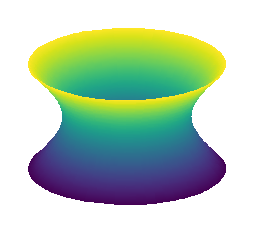
\begin{tikzpicture}[scale=0.5]
            \begin{axis}[
                    view={30}{30},
                    axis lines=none,
                    colormap/viridis,
                    samples=60,
                    domain=-1:1,
                    y domain=-2*pi:2*pi
            ]
            \addplot3[
                    surf,
                    shader=interp,
                    z buffer=sort
            ] ({0.2+cosh(x)*cos(deg(y))},
            {0.2+cosh(x)*sin(deg(y))},
            {sinh(x)});     
            \end{axis}
        \end{tikzpicture}
        \caption{Negative curvature}
     \end{subfigure}
     \hfill
     \begin{subfigure}{0.2\textwidth}
        \centering
        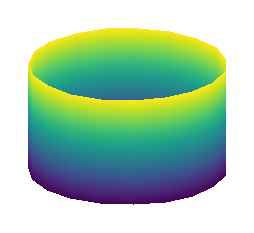
\begin{tikzpicture}[scale=0.5]
            \begin{axis}[
                    view={30}{30},
                    axis lines=none,
                    colormap/viridis,
                    samples=20,
                    domain=0:2*pi,
                    y domain=-1.5:1.5
            ]
            \addplot3[
                    surf,
                    shader=interp,
                    z buffer=sort
            ] ({cos(deg(x))},
            {sin(deg(x))},
            {y});
            \end{axis}
        \end{tikzpicture}
        \caption{Zero curvature.}
     \end{subfigure}
     \hfill
     \begin{subfigure}{0.2\textwidth}
        \centering
        
\begin{tikzpicture}[scale=0.5]
            \begin{axis}[
                    view={30}{0},
                    axis lines=none,
                    colormap/viridis,
                    samples=20,
                    domain=-90:90,
                    y domain=0:360
            ]
            \addplot3[
                    surf,
                    shader=interp,
                    z buffer=sort
            ]
            ({cos(x)*cos(y)},
            {cos(x)*sin(y)},
            {sin(x)});
            \end{axis}
        \end{tikzpicture}
        \caption{Positive curvature}     
    \end{subfigure}
    \label{fig:spaceCurvatures}\
    \caption{Surfaces with various curvatures.}
\end{figure}. In negative curvature spaces, the space bends like a saddle and triangle angles sum to less than $\pi$. We show a section of a hyperbolic paraboloid (described by function $z=x^2-y^2$) in \Cref{fig:hyperbolicSpace}.

\begin{figure}
    \centering
    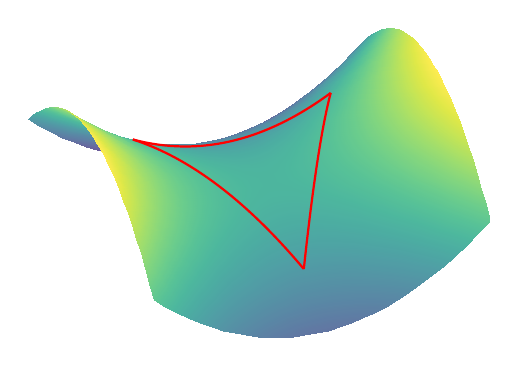
\begin{tikzpicture}
        \begin{axis}[
            view={160}{70},
            colormap/viridis,
            shader=interp,
            axis lines=none,
            xmin=-2, xmax=2,
            ymin=-2, ymax=2,
            zmin=-2, zmax=2,
        ]
        
        % Plot the hyperbolic paraboloid
        \addplot3[
            surf,
            domain=-1.7:1.7,
            domain y=-2:1.5,
            samples=30,
            opacity=0.8,
        ] {x^2 - y^2};
        
        % Define vertices of the triangle (lying on the surface)
        \newcommand{\vertexA}{(-1, -1, 0)}    % z = (-1)^2 - (-1)^2 = 0
        \newcommand{\vertexB}{(1, -1, 0)}     % z = 1^2 - (-1)^2 = 0
        \newcommand{\vertexC}{(0, 1, -1)}     % z = 0^2 - 1^2 = -1
        
        % Edge from A to B (along y = -1, z = x^2 - 1)
        \addplot3[
            thick,
            red,
            smooth,
            samples=50,
            samples y=0,
            domain=-1:1,
        ] ( 
            {x},                % x(x) = -1 → 1
            {-1},               % y(x) = -1 (consxanx)
            {x^2 - 1}         % z(x) = x(t)^2 - y(t)^2 = t^2 - 1
        );
        
        % Edge from A to C (parametric curve)
        \addplot3[
            thick,
            red,
            smooth,
            samples=50,
            samples y=0,
            domain=0:1,
        ] ( 
            {-1 + x},           % x(x) = -1 → 0
           { -1 + 2*x},         % y(x) = -1 → 1
            {(-1 + x)^2 - (-1 + 2*x)^2}  % z(x) = x(t)^2 - y(t)^2
        );
        
        % Edge from B to C (parametric curve)
        \addplot3[
            thick,
            red,
            smooth,
            samples=50,
            samples y=0,
            domain=0:1,
        ] ( 
            {1 - x},            % x(x) = 1 → 0
            {-1 + 2*x},         % y(x) = -1 → 1
            {(1 - x)^2 - (-1 + 2*x)^2}  % z(x) = x(t)^2 - y(t)^2
        );
        \end{axis}
        \end{tikzpicture}

    % 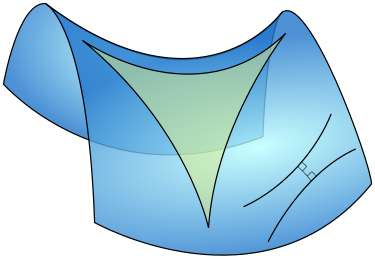
\includegraphics[width=0.3\textwidth]{figs/Hyperbolic_triangle.png}    
    \caption{Section of a hyperbolic space.}
    \label{fig:hyperbolicSpace}
\end{figure}




The induced distance between two points $(a,b)$ in $\mathbb{B}^d$ can be computed as
\begin{equation*}
    d_{\mathbb{B}}(a,b) = \text{arcosh}\left(1 + 2\frac{\|a-b\|^2_2}{(1-\|a\|^2_2)(1-\|b\|^2_2)}\right).
\end{equation*}
If $a = o$, the origin of the hyperbolic space, the distance function has the simple expression:
\begin{equation*}
    d_o(x) := d(o, x) = 2\tanh^{-1}(\|x\|_2).
\end{equation*}


An important concept in Euclidean geometry is that of straight lines, which are shortest paths between points. We can generalize this concept to manifolds by seeking curves with minimal length, called \term{geodesics}. The distance function induces two types of geodesics: straight lines that go through the origin and segments of circles perpendicular to the boundary of the ball (\Cref{fig:hyperbolicGeodesics}).
% Further, we can see from the distance formula that (Euclidean) norm-preserving transformations
% such as reflections, rotations centered at the origin and inversions are isometries of the hyperbolic
% space. We will extensively use these isometries throughout our work, especially inversions that map
% a reference point to the origin of the space.

%\begin{figure}
    \begin{subfigure}{0.48\textwidth}
        \centering
        \begin{tikzpicture}[scale=1.7]
            \draw (0,0) circle (1);
            \clip (0,0) circle (1);
            \hgline{30}{-30}{black!70}
            \hgline{180}{270}{blue!20}
            \hgline{30}{120}{black!70}
            \hgline{0}{180}{red!50}
        \end{tikzpicture}
        \caption{Poincaré ball model.}
        \label{fig:poincareBall}
    \end{subfigure}%
    \hfill
    \begin{subfigure}{0.48\textwidth}
        \centering
        \begin{tikzpicture}
        \begin{axis}[
            view={30}{10},
            colormap name=custom,
            shader=interp,
            axis lines=none,
            xmin=-3, xmax=3,
            ymin=-3, ymax=3,
            zmin=0, zmax=5,
        ]
        \addplot3[
            surf,
            domain=-2.8:2.8,
            y domain=-2.8:2.8,
            samples=20,
            z buffer=sort,
            opacity=0.7
        ] {sqrt(x^2 + y^2 + 1)};
        \end{axis}
        \end{tikzpicture}   
        \caption{Hyperboloid model.}
        \label{fig:hyperboloid}
    \end{subfigure}
    \caption{Models of hyperbolic space.}
    \label{fig:hyperbolicmodels}
\end{figure}


\subsection{Exponential and logarithmic maps}
For each point $p$ in a Riemannian manifold, the tangent space at $p$, $T_p$ is a $d$-dimensional vector space containing all possible directions of paths leaving from $p$. The tangent space maps to the manifold via the exponential map, and conversely, the logarithmic map translates the point on the manifold to the tangent space. In particular, we have closed-form expressions for these maps in the Poincaré ball when the reference point is the origin:
\begin{equation*}
    \exp_o(v) = \tanh(\|v\|) \frac{v}{\|v\|}
\end{equation*}
\begin{equation*}
    \log_o(y) = \text{arctanh}(\|y\|) \frac{y}{\|y\|}
\end{equation*}
Because the tangent space has a linear structure, we will rely on these maps to leverage some of the tools of Euclidean geometry for hyperbolic methods, such as optimization or neural network operations.

\section{Hyperbolic spaces and trees}


